%%%%%%%%%%%%%%%%%%%%%%%%%%%%%%%%%%%%%%%%%%%%%%%%%%%%
\graphicspath{{}{introduction/}{Diagrams/}}

These are exciting times in high-energy physics. The Standard Model (SM), our most powerful and well-tested theory of particles and their interactions, triumphs across the experimental landscape and proves to be much more robust than ever anticipated. Yet, as we will see throughout this thesis, once confronted with some of the simplest questions about the Universe, it provides unsatisfactory answers and, most surprisingly, little theoretical guidance on what may lie beyond. While there is no guarantee that the questions we ask are indeed ``good'' ones, to many, the limitations of the SM attest to the need of a new paradigm in particle physics. Whatever it may be, it makes the series of negative results in particle physics all the more thrilling. Uncertain moments like the one we live are frequent in the history of physics. For many times we saw established theoretical expectations and increasingly fine-tuned models making way for elegant theories like Special Relativity, for new particles such as the neutrino and for new ideas like spontaneous symmetry breaking (SSB).

In practice, of course, such grandiose endeavors are reduced to much less noble but no less important efforts. The frequency of negative results and the need to over-constrain our models make the search for new physics a true exercise in patience. Nevertheless, it is in a persistent and curious spirit that this thesis stands. The common theme of the work developed here is that of \emph{hidden neutrino physics}, both in the sense of rare neutrino processes and of hidden sectors beyond the SM. Hidden, dark or secret are all terms associated with new particles that hide not at high energies with $\mathscr{O}(1)$ couplings, but rather at lower scales with couplings to the SM that are much smaller than one. With the exciting theoretical and experimental prospects in neutrino and dark matter physics, we believe that it is all the more timely to think harder about what neutrinos, hidden particles of their own, may teach us about this type of hidden physics. 

We start this thesis by reminding ourselves of the main features and limitations of the SM in this chapter, and delving into unique aspects of neutrino physics in the next. This way, we hope to set the scene and motivate the direction we pursue in the following chapters. Indeed, the processes of neutrino trident production and neutrino-electron scattering we discuss in Chapter 3 are a testimony of the unique properties of neutrinos and the bright prospects in experimental neutrino physics. As a concrete example, we will see in Chapter 4 how such signatures probe new gauge interactions much weaker than those in the SM ($g \lesssim 10^{-3}$). The fact that neutrinos are the only neutral fermions in the SM also has interesting consequences for mass generation and naturally connects them to neutral hidden sectors. We explore this connection with a specific model at hand in Chapter 5, scrutinizing its phenomenology at short-baselines in Chapter 6. Finally, in Chapter 7 we look towards the far future and highlight the impact of a near-future entry-level neutrino factory in neutrino physics.

\section{The Standard Model}

The Standard Model (SM) of particle physics is a Yang-Mills theory~\cite{Yang:1954ek} of strong, weak and electromagnetic (EM) particle interactions based on an $SU(3) \times SU(2) \times U(1)$ local gauge symmetry. The first remarkable aspect of the theory is in the fact that it relies on the same idea that explains Maxwell's equations, the principle of gauge invariance. In this way, it is hard to pin down the official conception of the SM, although it is widely associated with the appearance of a model first developed by Sheldon L. Glashow~\cite{Glashow:1961tr}, Steven Weinberg~\cite{Weinberg:1967tq} and Abdus Salam~\cite{Salam:1968rm}. Unconcerned with quarks and the strong force, this spontaneously broken $SU(2) \times U(1)$ local gauge symmetry already reflected most of what we know about the electroweak (EW) interactions of leptons nowadays. In fact, the spontaneous broken symmetry that was used already predicted the existence of a charged massive vector boson, the $W^\pm$, a neutral massive vector boson, the $Z$, and of a massless generator of the unbroken $U(1)_{\rm EM}$ group, the photon $\gamma$. Beyond unifying the weak and EM forces, the breaking through the Higgs mechanism~\cite{Higgs:1964ia,Higgs:1964pj} implied that an additional scalar particle, the higgs boson $H$, had to exist. This last prediction was experimentally validated after the discovery of a neutral scalar boson at the LHC in 2012~\cite{Chatrchyan:2012xdj,Aad:2012tfa}, the last SM particle to be experimentally observed.

The strong force had a much richer and more turbulent history. The quark model, developed by Murray Gell-Mann and George Zweig~\cite{Zweig:1981pd,GellMann:1964nj} in 1964, had great success in explaining the growing number of hadronic resonances found by experiments. However, it was not until asymptotic freedom was discovered in non-Abelian gauge theories~\cite{Gross:1973id,Politzer:1973fx} that quantum chromodynamics (QCD) was really born. QCD is an $SU(3)$ local gauge theory describing the interaction of quarks and gluons, and is vastly different from any other theory we will encounter in this thesis. Its uniqueness is best exemplified through color confinement, the property that colored particles must always be present in bound colorless states, called hadrons. For QCD, confinement is guaranteed below the scale $\Lambda_{\rm QCD} \approx 250$ MeV, below which strong processes are non-perturbative. This is to be contrasted with asymptotic freedom, where the strong interactions between quarks and gluons become asymptotically weaker at higher energies. The presence of new degrees of freedom other than quarks and gluons at low energies, namely the hadrons, is a clear evidence of a phase transition and makes QCD a unique topic within the SM. At times we will refer to known results in this theory, but it usually has little bearings on electroweak physics.

\subsection{Fields and symmetries}

We now set out for a more precise definition of the SM field content, discussing some details of local gauge invariance. All fermion fields in the SM are Weyl fields of either definite left-handed (LH) or right-handed (RH) chirality. An equivalent statement is that SM fields are eigenvectors of $\gamma_5$: $\gamma_5 \psi_R = \psi_R$ for RH, and $\gamma_5 \psi_L = - \psi_L$ for LH fields. This is an important feature that allows us to work with 2 component Weyl spinors and makes explicitly manifest the chiral nature of weak interactions. The LH field content and their representation under the different gauge groups is shown in \reftab{tab:SMcharges}. Note that only LH particles transform non-trivially under $SU(2)_L$. Also shown is the Higgs field $H$, a complex scalar field, doublet under $SU(2)$. As we will see in the next section, $H$ is responsible for the breaking of $SU(2)_L \times U(1)_Y \to U(1)_{\rm EM}$.
%
\renewcommand{\arraystretch}{1.4}%
\begin{table}[t]
 \begin{tabular}{lccccccccccc}
 \hline
    & $Q_L^\alpha$& $L^\alpha$ & $\overline{u_R^\alpha\vphantom{d}}$ & $\overline{d_R^\alpha}$ & $\overline{e_R^\alpha\vphantom{d}}$ & &$H$ & & $G$ & $W$ & $B$\\
    \hline
  SU$(3)_c$ & $\bm{3}$ & $\bm{1}$& $\overline{\bm{3}}$ & $\overline{\bm{3}}$ & $\bm{1}$ & & $\bm{1}$ & & $\bm{8}$ & $\bm{1}$ & $\bm{1}$ \\
  SU$(2)_L$& $\bm{2}$ & $\bm{2}$ & $\bm{1}$ & $\bm{1}$& $\bm{1}$& & $\bm{2}$ & & $\bm{1}$ & $\bm{3}$ & $\bm{1}$ \\
  U$(1)_Y$ & $1/3$ & $-1$ & $-4/3$ & $2/3$ & $2$ & & $1$ & & $0$ & $0$ & $1$ \\
  \hline
 \end{tabular}
 \caption[SM field content.]{The representation of the SM left-handed Weyl fields, complex scalar and gauge bosons under each gauge group of the SM. For $U(1)_Y$, the charge is shown instead. All fermions carry a flavour index $\alpha = e, \mu$ or $\tau$.\label{tab:SMcharges}}
\end{table}
\renewcommand{\arraystretch}{1.0}%
%
From the observed EM charges $Q_{\rm EM}$, the $SU(2)_L$ isospin $T_3$, and by virtue of the Gell-Mann-Nishijima formula~\cite{Nakano:1953zz,Gell-Mann:1956iqa}
%
\begin{equation}
 Q_{\rm EM} = T_3 + \frac{Y}{2},
\end{equation}
%
the hypercharge $Y$ of each SM field is fixed. The \emph{local} gauge transformation of the matter fields are given by
\begin{equation}
\psi  \to \exp{i g \theta^a(x) T^a } \psi,
\end{equation}
where $g$ is the gauge coupling constant, $a$ counts the number of generators $T^a$, and $\theta^a(x)$ are arbitrary parameters that depend on space-time coordinates $x^\mu$. To achieve local gauge invariance, we require the following gauge fields associated with each group:
%
\begin{equation}
 SU(3)_C: \{G_1 (x), \cdots, G_8 (x)\}, \quad SU(2)_L:  \{W_1(x), W_2(x), W_3(x)\}, \quad U(1)_Y: B(x),
\end{equation}
%
corresponding to the eight gluons, the $SU(2)$ gauge fields and the hypercharge field. Note that the number of gauge fields matches the number of generators in each group, \eg\ for $SU(N)$ there are $N^2 -1$ generators. For the original $SU(2)\times U(1)$ theory, this implied that in addition to the charged gauge fields, which explained Fermi's theory for beta decays, and the observed massless photon, there must have been an additional neutral gauge field corresponding to some linear combination of $W^3$ of $SU(2)_L$ and $B$ of $U(1)_Y$. This striking prediction was in fact first confirmed by Gargamelle, a bubble chamber experiment, through the observation of accelerator neutrinos scattering into final states with no charged leptons~\cite{Hasert:1973ff}. 

The SM is a non-Abelian theory, since its symmetry group contains direct products of two $SU(N)$, $N > 1$, groups. The generators of a given group equipped with commutators form a Lie Algebra, obeying $[T^a, T^b] = i f^{abc} T_c$, with $f^{abc}$ being the group structure constant. In the special case $f^{abc} = 0$, the generators commute and the group is said to be Abelian, like in the case of $U(1)_Y$. Otherwise, the group is non-Abelian and the theory displays a much richer underlying dynamics. Take an $a$-dimensional Yang-Mills theory and define $\bm{\theta} = T^a \theta^a$ and $U = e^{i g \bm{\theta}}$. We can now perform gauge transformations on the relevant matter fields $\psi$, gauge fields $\bm{A}_\mu = T_a A_\mu(x)^a$ and derivatives of matter fields as follows
%
\begin{equation}
\psi \to U \psi, \quad \bm{A}_\mu \to U \bm{A}_\mu U^{-1} - \frac{i}{g} (\partial_\mu U) U^{-1}, \quad \partial_\mu \psi \to U \partial_\mu \psi +  \psi (\partial_\mu U).
\end{equation}
%
As we can see, the last term is not invariant due to the local character of the gauge transformations. To preserve gauge invariance, a covariant derivative, transforming as $D_\mu \to U D_\mu U^{-1}$, now replaces the ordinary derivative. It is defined as 
\begin{equation}
D_\mu = \partial_\mu + ig \bm{A},\quad \text{such that} \quad D_\mu\psi \to U D_\mu\psi, \,\,\implies\,\,\overline{\psi} i\slashed{D}\psi \to \overline{\psi} i \slashed{D} \psi. 
\end{equation}
%
The invariant term above is the fermion kinetic term. Beyond fermion propagation, it is the main way to describe fermion-gauge interactions in the SM. In particular, the full covariant derivative in the SM is given by
%
\begin{equation}
 D_\mu = \partial_\mu + ig \,W_\mu^a\tau_a + i\frac{Y}{2} g^\prime \,B_\mu + i\frac{g_s}{2} \,G_\mu^b\lambda_b,
\end{equation}
%
where $\tau_a = \sigma_a/2$ are the generators built from Pauli matrices acting on the doublets of $SU(2)_L$, and $\lambda_b$ the generators built from the Gell-Mann matrices acting on the triplet representations of $SU(3)_c$. The factors of $1/2$ come from the canonical  This also fixes the different gauge couplings of the SM. Finally, the gauge invariant kinetic terms for the gauge bosons are 
%
\begin{equation}
\mathscr{L}_{\rm Gauge} = -\frac{1}{4} G^{a}_{\mu\nu} G_a^{\mu\nu} - \frac{1}{4} W^{a}_{\mu\nu} W_a^{\mu\nu} -\frac{1}{4} B_{\mu\nu} B^{\mu\nu},
\end{equation}
%
where $F^a_{\mu \nu} = \partial_\mu F^a_\nu - \partial_\nu F^a_{\mu} - g_F f^{abc} F_{b\,\mu} F_{c\,\nu}$ with $g_F$ the relevant gauge coupling. The kinetic term in Abelian theories concern only the propagation of gauge bosons, however, for non-Abelian groups the term proportional to $g_F$ in $F^a_{\mu \nu}$ introduces interactions among the gauge bosons proportional to $g$ and $g^2$. Therefore, a non-Abelian theory is already an interacting theory without the addition of any matter fields.


\subsection{Spontaneous symmetry breaking}

So far we have only discussed the gauge and fermionic content of the SM. The scalar sector is, in fact, quite special. The only scalar particle, the higgs boson, is responsible for spontaneously breaking $SU(2)_L\times U(1)_Y$ to $U(1)_{\rm EM}$ after it acquires a non-zero vacuum expectation value (vev). This introduces a mass scale in the theory which, apart from dimensionless couplings, sets the scale of EW physics. Note that because it is a scalar particle, a non-zero vev does not violate the symmetries of space-time, namely Lorentz invariance. The higgs is a complex scalar field and a doublet under  $SU(2)_L$, and so we can write
%
\begin{equation}
  H =  \frac{1}{\sqrt{2}} \left( \begin{matrix}  G_1^+ + i G_2^+ \\  h^0 + i G_3^0 \end{matrix} \right) =  \frac{e^{i G_a \tau^a}}{\sqrt{2}} \left( \begin{matrix} 0 \\  h \end{matrix} \right).
\end{equation}
%
The relevant Lagrangian in the SM reads
%
\begin{equation}
\mathscr{L}_{\rm higgs} \supset \left( D^\mu H \right)^\dagger \left( D_\mu H \right) - V(H), \qquad V(H) = \mu^2 H^\dagger H + \lambda \left( H^\dagger H \right)^2.	
\end{equation}
%
where $\mu^2$ has mass dimension 2, being the only dimensionful parameter in the SM. If $\mu^2 < 0$, minimizing the potential $V(H)$ requires $\bra{0} H \ket{0} = \left( 0, \,\, v/\sqrt{2} \right)^T$, where $v^2 = - \mu^2 /\lambda$ is the vev chosen to lie in the real and neutral direction. We now can then expand around the true vacuum of the theory by redefining the fields $G_a \to G_a/v$ and $h \to h + v$. At this point, a rewriting of the potential reveals the mass and interactions of every component of the scalar doublet. Note, however, that it contains no mass terms for $G_1$, $G_2$ and $G_3$. These are the Goldstone bosons of the theory, and although they are massless, they do possess interactions with the scalar and gauge boson fields. One way to understand their role is to perform an $SU(2)_L \times U(1)_Y$ gauge transformation in our Lagrangian such that the resulting higgs doublet reads
%
\begin{equation}
H \to e^{- i G_a \tau^a/v} H =  \frac{1}{\sqrt{2}}\left( \begin{matrix}  0 \\ h + v \end{matrix} \right).
\end{equation}
%
This transformation must also be applied to the gauge fields, fixing the gauge. This particular choice is rather convenient and is known as the unitary gauge. We then find
%
\begin{align}
 \mathscr{L}_{\rm higgs} &\supset - \frac{1}{2} m_h^2 h^2 - \lambda v h^3 - \frac{\lambda}{4} h^4  \nonumber\\ &\qquad\qquad +  M_\textsc{w}^2 W_\mu^\dagger W^\mu \left[ 1 + \frac{2 h}{v} + \frac{h^2}{v^2}\right] + \frac{M_\textsc{z}^2}{2} Z_\mu Z^\mu \left[ 1 + \frac{2 h}{v} + \frac{h^2}{v^2}\right],
\end{align}
%
where $m_h = \sqrt{2\lambda}\, v = 125.18 \pm 0.16$ GeV~\cite{PDG}. Most importantly, after SSB, the higgs kinetic term has given us three massive and one massless vector bosons, defined as
\begin{equation}
 W^\pm_\mu = \frac{1}{\sqrt{2}} \left(W^1_{\mu} \mp i W^2_{\mu} \right), \quad Z_\mu = c_\textsc{w} W^3_\mu - s_\textsc{w} B_\mu, \quad A_\mu = c_\textsc{w} B_\mu - s_\textsc{w} W^3_\mu.
\end{equation}
% 
where $s_\textsc{w}$ ($c_\textsc{w}$) is the sine (cosine) of the weak angle, defined by $c_\textsc{w} = g/\sqrt{g^2 + g^{\prime\,2}}$. These fields correspond to the mediators of the weak charged-current interactions ($M_\textsc{W} = g v/2 = 80.387\pm 0.016$ GeV~\cite{PDG}), weak neutral-current ($M_\textsc{z} = M_\textsc{w}/c_\textsc{w} = 91.1876\pm0.0021$ GeV~\cite{ALEPH:2005ab}) neutral boson and the massless photon $A_\mu$, mediator of the unbroken EM interactions. They interact with the higgs boson via the triple and quadruple vertex terms above. The interactions with matter are obtained from the fermion kinetic terms, where the charged, neutral and electromagnetic currents are defined and written as
%
\begin{equation*}
\mathscr{L}_{\rm NC} = e \,{J}_\mu^\gamma A^\mu + \frac{g}{c_\textsc{w}}\, {J}_\mu^Z Z^\mu, \quad {J}_\mu^\gamma =  \overline{\psi} Q_{\rm EM} \gamma_\mu \psi, \quad %
{J}_\mu^Z = \overline{\psi} \gamma_\mu \left[ \left( \frac{T_3}{2} - Q_{\rm EM} s_\textsc{w}^2 \right) - \frac{T_3}{2} \gamma^5\right] \psi,
\end{equation*}
\begin{equation}
\mathscr{L}_{\rm CC} = \frac{g}{\sqrt{2}}  \, \left( {J}_\mu^+ W^{\mu \,+} + {J}_\mu^- W^{\mu \,-} \right), \quad
%
{J}_\mu^+ = \frac{1}{2} \overline{\psi}_u \gamma_\mu \left( 1 - \gamma^5\right) \psi_d + {\rm h.c.},
\end{equation}
%
where $\psi \in \{ \nu_L, e_L, u_L, d_L, e_R, u_R, d_R \}$, and $\psi_{u,\,d}$ denoting fermions with $T_3 = \pm 1/2$. From the weak currents we note two important aspects: \emph{i)} weak interactions indeed violate parity and possess a $V-A$ structure, \emph{ii)} charged-current interactions are purely LH as they should be since no RH fields are charged under $SU(2)_L$. After SSB, only the EM current is conserved $\partial^\mu J_\mu^\gamma = 0$. 

In the discussion above, we fixed the gauge of the SM to simplify the EW Lagrangian. This is not necessary and, in fact, another possibility is to keep all terms involving the Goldstone fields $G_a$ and eliminate off-diagonal kinetic terms of the type $Z_\mu\partial^\mu G_3$ by introducing the following gauge breaking Lagrangian to the SM
\begin{equation}
 \mathscr{L}_{\rm R_\xi} = -\frac{\left(\partial_\mu A^\mu\right)^2}{2 \xi_\gamma} - \frac{\left(\partial_\mu Z^\mu + \xi_Z M_Z G_3^0 \right)^2}{2 \xi_Z} - \frac{\left|\partial_\mu W^{\mu\,-} + i \xi_W M_W G^- \right|^2}{2 \xi_W}.
\end{equation}
This is known as the $R_\xi$ gauge, where the explicit dependence on the gauge breaking parameters $\xi$ serves as a useful diagnostic of gauge invariance in physical observables. The Lorentz gauge is recovered for $\xi = 0$ and the Feynman-'t Hooft gauge with $\xi = 1$. The additional advantage of using this method is that it allows us to trace the Goldstone degrees of freedom. The pseudoscalar fields $G^\pm$ and $G_3$ end up behaving very similarly to the $W^\pm$ and $Z$ gauge bosons. In fact, at high-energies it can be shown that the Goldstone bosons are equivalent to the longitudinal polarization states of their respective gauge bosons~~\cite{Cornwall:1974km,LlewellynSmith:1973yud}. This is known as the Goldstone boson equivalence theorem, and it turns out to be very important to understand processes like $W_L \, W_L$ and $Z_L \,Z_L$ scattering. At very high-energies and without the Higgs boson, such processes grow indefinitely ($\sigma \propto s$), spoiling the unitarity of the $S$-matrix. The fact that this problem was solved by including contributions from $h$ exchange provided a no-lose theorem for the LHC: either the higgs boson would be discovered, or new physics must appear to unitarize these processes. 

\subsection{Fermion masses}

The EW sector is also responsible for the generation of fermion masses in the SM. As noted before, all LH fermions in the SM are $SU(2)_L$ doublets, just like the higgs. This allows us to construct the so-called Yukawa terms,
%
\begin{equation}
 \mathscr{L}_{\rm Yukawa} =  y_e \left(\overline{L}_\alpha H\right) e_R +  y_u \left(\overline{Q}_L \tilde{H} \right) u_R + y_d \left(\overline{Q}_L H \right) d_R  + \,\, {\rm h.c.},
\end{equation}
%
where we defined the charge-parity (CP) conjugated higgs field $\tilde{H} = i \sigma_2 H^* = ( h + v + i G_3, \,\, G_1 - i G_2  )^T$. After SSB, these interaction terms endow charged-leptons and quarks with a dirac mass term of the form
\begin{equation}
 m_\psi \overline{\psi} \psi = m_\psi \left( \overline{\psi}_L \psi_R +\overline{\psi}_R \psi_L \right),\quad {\rm with} \quad m_\psi = \frac{y_\psi \, v}{2},
\end{equation}
where $\psi_{L,\,R} = P_{L,\, R} \, \psi = (1 \mp \gamma_5)\, \psi/2 $ are the chiral projections of the fermion field $\psi$. To include all three families of fermions we promote $y_\psi \to \bm{y}_\psi$, a $3\times3$ matrix. 

In the quark sector, the Yukawa matrix is off-diagonal and the different generations mix. The physical quark masses are found after rotating the up and down quarks, left and right, as $u_{L,\, R}^\alpha = \left(V_{L,\,R}^{u\,*} \right)_{\alpha i} u^i_{L,\, R}$ and $d_{L,\, R}^\alpha = \left(V_{L,\,R}^{d\,*} \right)_{\alpha i} d^i_{L,\, R}$. The diagonal mass matrix is then $\bm{m}^{u,\,d} = \bm{V}_L^{u,\,d} \bm{y}_{u,\,d} \bm{V}_R^{u,\, d\,\dagger} v/\sqrt{2}$. Note that after this procedure we cannot help but introduce mixing in the charged current. This defines the Cabbibo-Kobayashi-Maskawa (CKM) matrix~\cite{Cabibbo:1963yz,Kobayashi:1973fv}, $\bm{V}_{\rm CKM} = \bm{V}_L^u \bm{V}_L^{d\, \dagger}$. The CKM matrix is nearly diagonal, so the mixing between quark flavour and mass eigenstates is small. From the unitarity of the rotation matrices, neutral currents remain invariant 
\begin{equation}
\sum_{\alpha,\, \beta} \overline{\psi}_L^\alpha \,\Gamma^\mu \, \psi_L^\beta = \sum_{i,\,j} \overline{\psi}_L^i \, \left( \sum_{\alpha,\, \beta} (V_L)_{\alpha i} (V_L^*)_{\beta j}\right) \,\Gamma^\mu\, \psi_L^j =  \sum_{i,\,j} \overline{\psi}_L^i \, \,\Gamma^\mu\, \psi_L^j,
\end{equation}
%
where $\Gamma^\mu$ are the neutral-current couplings and gamma matrices.  Crucially, the latter have no flavour dependence and so the SM forbids flavour changing neutral currents (FCNC). This mechanism was first proposed by Glashow, Illiopoulous and Maiani to explain why decays of the type $K^0 \to \mu \mu$ were unobserved. Famously referred to as the GIM mechanism, this relies on the flavour universal nature of SM neutral currents and on the unitarity of the CKM. As we will see, this mechanism also plays an important role in the neutrino sector and in many extensions of the SM.

Summarizing, we saw how a single parameter with massive dimensions in the scalar potential of the SM leads to SSB. This is then ``propagated'' to the rest of the SM through the higgs kinetic terms and Yukawa couplings. At this point it is possible to appreciate two problems with the SM mass generation mechanism. Firstly, it implies that all Yukawa couplings are just parameters to be inferred from the measured masses of particles. That is, the SM makes no statements and provides no explanations as to why the Yukawas that we observe in nature are what they are. This is known as the flavour puzzle: what explains the different observed values of the fermion masses? This problem is aggravated when we consider the lepton sector, where neutrino masses and mixing are drastically different from the quark sector. The second problem concerns the neutrino sector, and is perhaps the biggest motivation behing studying neutrino physics. The SM predicts exaclty massless neutrinos in the absence of $\nu_R$ fields. Although  

Before moving on to more speculative topics, a few comments are in order. EW SSB seems to be, as far as we know, a real phenomenon. It explains why the symmetries of the SM were so well hidden the first place: true symmetries of Nature seem to not be shared by the vacuum. While the evidence for EW SSB comes mainly from studying fundamental particles, its consequences do not concern only particle physics. EW physics helps us understand the past and future of our own Universe. In the early Universe, at hight temperatures, it is expected that the EW symmetry is restored~\cite{Kirzhnits:1972ut,Dolan:1973qd,Weinberg:1974hy}. If this is the case, the EW phase transition provides a unique test of the higgs mechanism and points to a completely different Universe from our own, where finite temperature effects and non-perturbative physics play a major role. In addition, we have no reason to expect the vacuum structure of the Universe to be as simple as in the discussion above. After all, the stability of our own vacuum is not even guaranteed within the SM~\cite{Cabibbo:1979ay,Degrassi:2012ry}. Radiative corrections to the higgs self-coupling $\lambda$ alter the shape of the scalar potential and imply we may live in a local, rather than global, minimum of the potential. For these reasons, studying the higgs sector, confirming that it generates all fermion masses in the SM and why it seemingly fails to do so in the case of the neutrino are all important questions worth pursuing.

\begin{figure}
 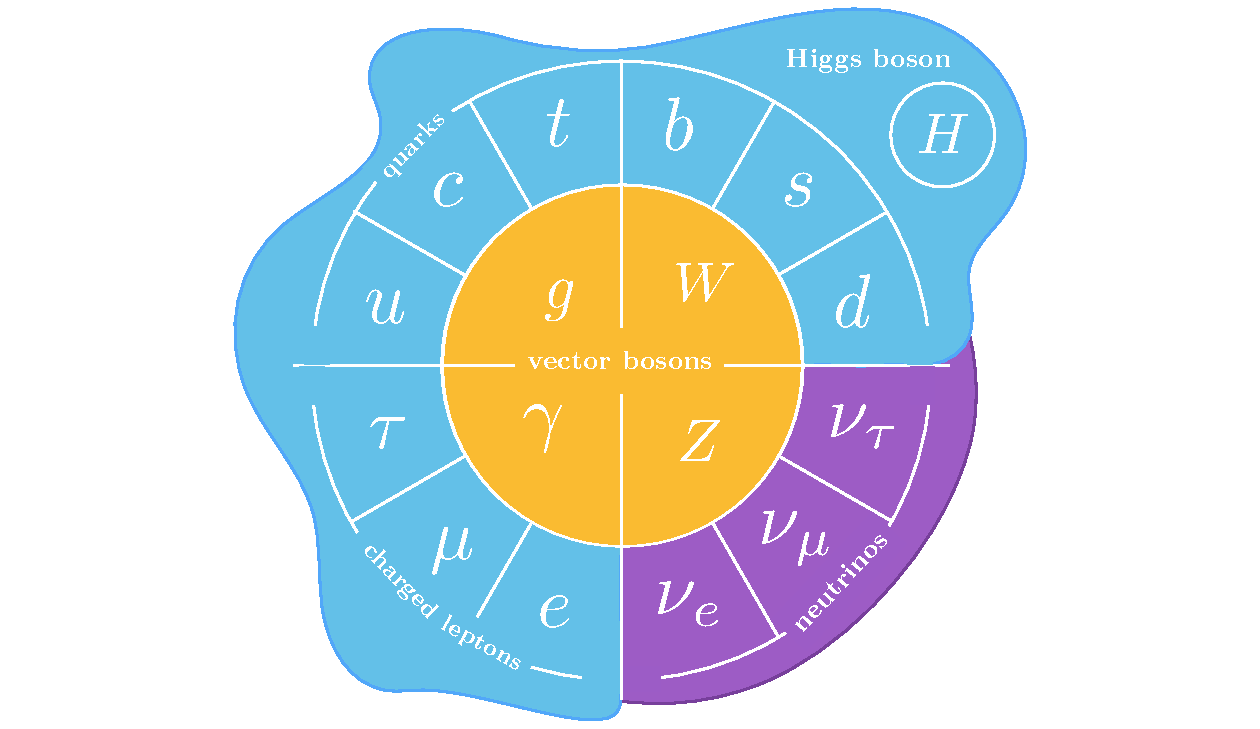
\includegraphics[width=0.96\textwidth]{SM_zoo.pdf}
 \caption{Artistic rendering of the particles in the Standard Model. \label{fig:SM_diagram}}
\end{figure}



%%%%%%%%%%%%%%%%%%%%%%%%%%%%%%%%%%%%%%%%%%%%%%%%%%%%%%%%%%%%%%%%%%%%%%%%%%%%%%%%
%
% BSM!!!!!!
%
%%%%%%%%%%%%%%%%%%%%%%%%%%%%%%%%%%%%%%%%%%%%%%%%%%%%%%%%%%%%%%%%%%%%%%%%%%%%%%%

\section{Evidence for Beyond the Standard Model physics}

The most important building aspects and building blocks of the SM have been laid out above. Now, a different question will concern us: is this theory sufficient to explain fundamental particles and their interactions? We have already stumbled upon a few problems of the SM, but even before that one must already suspect that the SM is not a final theory. It does not explain gravity. This tells us that the SM should be treated as an effective theory valid up until the Planck mass $M_{\rm Pl} = \left(\hbar c/ 2 G_{\rm Newton}\right)^{1/2} \approx 10^{19}$ GeV, where the effects of gravity are expected to be large~\footnote{This is a naive expectation based on the observation that the Schwarzschild radius $\ell_s = 2 G_{\rm Newton} m/c^2$ and the Compton wavelength $\ell_c = h /mc$ of a particle become comparable at $m \approx M_{\rm Pl}$.}. This very own fact already brings us to one of the most controversial evidences for beyond the Standard Model (BSM) physics.

\paragraph{The hierarchy problem} The lack of evidence for new physics at the LHC can be argued to be more than just unfortunate. If no new physics is indeed present between the EW and the Planck scale, then the cut-off of the SM, beyond which the effective field theory is no longer valid, is $\Lambda = M_{\rm Pl}$. This implies that unless symmetries are at play, terms of dimensions $d$ are suppressed or are of the order of $\Lambda^{4-d}$. However, in the SM $m_h^2 \ll \Lambda$, suggesting a fine-tuning of many orders of magnitude. Quantum corrections to the higgs mass, $m_h^2 = m^2_{\rm bare} + \delta m_h^2$, are dominated by the top quark and go as $\delta m_h^2 = y_t^2 \Lambda^2 / 8 \pi^2$. This quadratically divergent result implies that to obtain the observed light higgs mass, whatever new physics that may appear at the scale $\Lambda$ (possibly even below $M_{\rm Pl}$) must cancel the fermion loops to order $m_h^2/ \Lambda^2$. In other words, the matching condition for the renormalization of $m_h^2$ parameter becomes fine-tuned to order $m_h^2/ \Lambda^2$ in the presence of such cut-off. Supersymmetric theories are notorious candidates that solve this problem, but so far we are yet to find any evidence for them. One may argue that indeed there exists a ``desert'' between the EW and the Planck scale, and that some miraculous mechanism is at play in quantum gravity that may solve the fine-tuning problem. In that case, a solution to all following items in this list must be found there, or somewhere outside the realm of particle physics.

\paragraph{The strong-CP problem} The QCD Lagrangian admits the following field-strength contraction term
%
\begin{equation}
 \mathscr{L} \supset \frac{\theta \alpha_s^2}{8\pi} G_{\mu\nu}^a \tilde{G}_a^{\mu\nu},\quad {\rm where }  \quad \tilde{G}^a_{\mu\nu} = \frac{\epsilon_{\mu\nu\rho\sigma}}{2} {G}^{a\, \rho\sigma}.
\end{equation} 
This can be shown to be a surface term (a total divergence in the action) and can be neglected in perturbative calculations. Nevertheless, this term induces CP violation in the strong sector via non-perturbative effects, leading to a large electric dipole moment for free neutrons~\cite{Crewther:1979pi}, which is orders of magnitude above the experimental upper limits~\cite{Afach:2015sja}. The most popular scenario to explain the smallness of $\theta$ is the Peccei-Quinn symmetry~\cite{Peccei:1977ur}, a global chiral $U(1)$. The breaking of this symmetry leads to the prediction of a Goldstone boson, the axion.

\paragraph{Matter-antimatter asymmetry} The observed baryon asymmetry of the Universe contradicts the standard Cosmology, which predicts that matter and anti-matter were created in equal amounts in the Big Bang. The SM does not provide enough source of CP violation to explain this phenomenon. Popular scenarios to explain this are EW baryogenesis and Leptogenesis, where the latter relies on the CP violation from a heavy neutrino sector and its translation into a baryon asymmetry through Spharelon processes.

\paragraph{Dark matter} Measurements of the redshift of galaxy clusters in the 1930's~\cite{Zwicky:1933gu} and galaxy rotation curves in the 70's~\cite{Rubin:1970zza}, are among the pioneering work that showed that the gravitational potential in such astrophysical scales is much deeper than the one extrapolated from luminous matter. Already at the time, astronomers would refer to the source of this additional gravitational influence as Dark Matter (DM). As Astrophysics and Cosmology evolved, concrete evidence for DM continued to build up. Evidence for DM is now present at a variety of scales, from the precise measurements of the cosmic microwave background (CMB)~\cite{Akrami:2018vks}, the matter distribution in galaxy cluster mergers~\cite{Clowe:2006eq}, and the observed large scale structure of the Universe~\cite{Blumenthal:1984bp}. In fact, from CMB power spectrum we can infer the DM density today as~\cite{Akrami:2018vks}
\begin{equation}
 \Omega_{\rm DM} h^2 = 0.1200\pm0.0012
\end{equation}
with $\Omega_{\rm DM} = \rho_{\rm DM}/\rho_c$ the energy density of DM in units of the critical density $\rho_c \approx 10^{-26}$ kg/m$^3$, and $h = H_0/(100$ km s$^{-1}$/Mpc$^{-1}) = 0.674\pm0.005$ the scaled Hubble expansion rate. This is roughly five times larger than the density of baryons, understood as all other non-relativistic matter. The latter is also measured through the relative abundances of light elements during Big Bang Nucleosynthesis (BBN)~\cite{Cooke:2013cba}, where DM plays no role and providing further evidence for non-baryonic DM.

The nature of DM is not yet understood and many possibilities are under discussion. Modified gravity models explain local astrophysical observations, but struggle to explain all CMB datasets and X-ray observations of mergers of galaxy clusters~\cite{Famaey:2011kh}. Primordial black holes~\cite{Barack:2018yly} have also been put forward as DM candidates and have triggered great interest due to their connection to the detection of gravitational waves. However, the most popular hypothesis at this point remains that DM is made of new particles. This new state better be neutral, to have evaded our detection, and sufficiently long-lived, so that it may linger until today after its production in the early Universe. The fluid of such particles would have to display negligible pressure and viscosity, and to have been created cold so as to help form clumpy structures in the Universe with its gravitational influence. This points us to a particle that is massive, collisionless and, yet, very abundant today. Most notably, DM models have often focused on the possibility of a weakly-interacting massive particle (WIMP). In this paradigm, DM particles, say $\chi$, are produced in the early Universe through its weak interactions with the SM plasma. At later times, approximately at temperatures of the order of the DM mass $m_{\chi}$, DM production stops and annihilation into SM particles dominates. As the Universe cools and expands, the DM gas is diluted and annihilation is no longer effective, \emph{freezing-out} the DM population at around $T \approx m_{\chi}/20$. In particular, the relic density obtained in this mechanism is of the order $\Omega_\chi H_0^2 \approx 0.1 \,{\rm pb}/ \sigma$, where $\sigma$ stands for the thermally averaged cross section of $\chi$ annihilation into SM particles. The fact that $\sigma\approx 1$ pb allows to reproduce the current DM density and is of the order of typical weak cross sections (as in mediated by weak bosons) is known as the WIMP-miracle. WIMP DM is a collisionless and thermal candidate, although DM candidates that are non-thermal, or collisionless, or both exist.

\paragraph{Neutrino masses} One of the most important evidences for BSM physics is the fact that neutrinos have mass. This comes from the plethora of experimental evidence for neutrino oscillations, which we explore in the next chapter. Put simply, neutrino oscillation data requires at least 2 non-zero and non-degenerate massive neutrinos. Although one might argue that this is solved by the mere addition of at least 2 RH neutrino states to the SM which are complete singlets of the symmetry, this simple extension still requires further study and experimental confirmation. In addition, such states would be the only SM particle to admit a Majorana mass term of the type $M \,\overline{\nu^c}_R \nu_R$, and unless new symmetries are introduced, there is no reason to expect that $M$ is exactly zero. Therefore, it is customary to think that neutrino masses are the first indications of physics beyond the SM observed in controlled laboratory conditions.   

\section{Extending the Standard Model}

In extending the SM one may take several approaches. We can be guided by experimental results and tensions, by increased symmetries and elegance in our theories, or by complete agnosticism. While we lack a single compelling evidence for the direct detection of a new particle, we can interpret many of the problems outlined above as evidence for new states. The existence of DM and neutrino masses, in particular, suggests (but does not require) that these new states may be a new sector of electromagnetically neutral particles. Here, the SM provides no guidance for their masses or symmetries, and so a mixture of all three approaches outlined before is common in the literature. This thesis is no exception.

Dark sectors are a typical prediction of theories with 


Our BSM extensions all involve light and hidden new states, which have evaded detection to the smallness of their couplings to the SM. This point of view is compelling from a DM and neutrino perspective.

only neutral particle in the SM , in the spotlight 

In this sense, our job is to search ``under the lightpost'', using current and future experiments to look for new physics in a opportunistic way. Not only is this a cheap and viable exercise, it would offers an explanation as to why the SM performs so well as a theory and against most experimental tests. A modular view of the Universe, with the visible SM sector and potential dark sectors barely influencing each other wou

Given the hints that dark sectors beyond the SM may exist, we would like to investigate all the possible ways the particles in this sector may interact with the SM. One way to tackle this question is to build effective field theories, where one studies all operators which are allowed by the content and symmetries of the SM. The idea is to construct a series of $d>4$ operators in $1/\Lambda^{d-4}$, where $\Lambda$ is the scale of the new physics. This approach thrives on its generality, but can become complicated very quickly with growing $d$. Most importantly, the scale $\Lambda$ is assumed to be large, so that all new degrees of freedom have been integrated out of the theory. This is suitable for extensions involving particles which are very heavy, but the series is no longer well defined for new physics that is light and kinematically accessible at our experiments. In this case, the kinematics of the new particles play a role, forcing us to write down the field content and symmetry group of the new physics. This is the approach we will follow in this thesis.

\subsection{Portals to hidden sectors}

We would like our SM extensions to follow specific guiding principles and organize them in a meaningful way. One way to do so is to study all the low dimension neutral operators that the SM has to offer. In contrast to effective field theories, we want renormalizable operators with $d<4$ which are also gauge invariant. As it turns only a few such operators exist, which we usually refer to as \emph{portals}. We dedicate this section to presenting these.

\paragraph{Neutrino portal} Arguably the most motivated portal, this $d=5/2$ operator can be written as
\begin{equation}
\left( \overline{L}^\alpha_a \cdot \tilde{H}\right), %= \left( \left(\nu^\alpha_L\right)_a \,\, \left(e_L\right)_a \right)
\end{equation}
%
where we made the spinor index $a$ explicit. Any fermion field which couples to this operator acquires couplings to SM neutrinos. This typically induces off-diagonal mass terms in the Lagrangian, leading to mixing between the new species and all massive neutrinos in the broken phase of the SM. The new particle is then commonly referred to as \emph{heavy neutral lepton} or right-handed neutrino, though its chirality is a matter of convention.

\paragraph{Vector portal} Any new vector particle $X^\mu$ may couple to the $d=2$ field strength of the SM hypercharge
\begin{equation}
B_{\mu\nu},
\end{equation}
through its own field strength tensor $X^{\mu\nu}$. The resulting term, $B_{\mu\nu} X^{\mu\nu}$, is a off-diagonal kinetic term for the massive bosons and is sometimes called the \emph{kinetic mixing} operator. To work in a basis of physical states with diagonal kinetic terms, where the propagators are in their standard form, one usually performs a field redefinition. If much lighter than the EW scale, the new vector particle couples primarily to the EM current, hence the name dark photon. If heavy, it can also couple to the NC and is therefore referred to as a dark $Z$. Models with the term 
%
\begin{equation}
 Z_\mu X^\mu 
\end{equation}
%
also come up in the literature, where it is said that \emph{mass-mixing} between the new vector particle and the SM $Z$ exists. This term is not gauge invariant, but may arise in the broken phase of BSM theories with additional doublet scalars, like in two-higgs-doublet models (2HDM). In this case, several charged degrees of freedom typically appear and experimental constraints tend to be more severe.

\paragraph{Higgs portal} New scalar particles can couple to the $d=2$ bilinear 
%
\begin{equation}
 H^\dagger H,
\end{equation}
%
the only renormalizable portal with no free Lorentz or spinor indices. In this case there are two possibilities for a scalar to couple to the SM, depending on its charges. We can write  $H^\dagger H \, S^\dagger S$ for a charged, or $H^\dagger H\, S $ for a singlet complex scalar. The latter term is the only super-renormalizable operator connecting the SM fields to new physics which is allowed. Beyond important consequences for EW SSB, these operators typically inherit the higgs couplings to matter fields, and may be hard to search for due to the smallness of the SM Yukawa couplings. A very simple BSM model with such portal arises in scalar singlet $S$ extensions, where one generates the term $H^\dagger H \, S^\dagger S$~\cite{Silveira:1985rk}. Remarkably, this extension can also have consequences to the "little hierarchy" problem, as the new scalar also contributes to the Higgs self-energy~\cite{Craig:2013xia}.


\paragraph{Fermionic currents}

A whole set of neutral operators in the SM come from the fermionic currents
\begin{equation}
 J^\mu \equiv \overline{\Psi} \gamma^\mu \Psi,
\end{equation}
where $\Psi \in \{Q_L, L, u_R, d_R, \ell_R\}$. This provides SM currents which can be associated with new conserved charges, which in turn may be promoted to a local or global gauge symmetry. The first condition is that it be locally conserved $\partial_\mu J^\mu = 0$. 

\paragraph{Pseudo-scalar} Axions~\cite{Weinberg:1977ma}.




